\documentclass[12pt]{book}
\usepackage[utf8]{inputenc}
\usepackage[T1]{fontenc}
\usepackage{amsmath}
\usepackage{amssymb}
\usepackage{geometry}
\usepackage{tikz}
\usepackage{pgfplots}
\usepackage{xcolor}
\usepackage{mdframed}
\usepackage{enumitem}
\usepackage{booktabs}
\usepackage{array}
\usepackage{fancyhdr}
\usepackage{titlesec}
\pgfplotsset{compat=1.18}
\geometry{margin=1.1in, top=1.2in, bottom=1.2in}

\definecolor{mathblue}{RGB}{30,90,160}
\definecolor{mathgreen}{RGB}{30,140,80}
\definecolor{mathred}{RGB}{180,40,40}
\definecolor{lightgray}{RGB}{240,240,240}

\titleformat{\chapter}[display]
  {\normalfont\large\bfseries}
  {\chaptertitlename\ \thechapter}{12pt}{\LARGE}
\titleformat{\section}
  {\normalfont\large\bfseries}{{\thesection}}{1em}{}
\titleformat{\subsection}
  {\normalfont\normalsize\bfseries}{{\thesubsection}}{1em}{}

\setcounter{chapter}{2}

\pagestyle{fancy}
\fancyhf{}
\fancyhead[LE]{\small\textit{Chapter \thechapter.\ Basic Statistics}}
\fancyhead[RO]{\small\textit{Observing with Mathematical Perspectives}}
\fancyfoot[C]{\small\thepage}
\renewcommand{\headrulewidth}{0.4pt}

\newcounter{exercise}[section]
\renewcommand{\theexercise}{\thesection.\arabic{exercise}}
\newenvironment{exercises}{%
  \begin{mdframed}[backgroundcolor=lightgray, linewidth=0pt,
    innertopmargin=10pt, innerbottommargin=10pt]
  \noindent\textbf{Exercises \thesection}
  \begin{list}{\theexercise.}
    {\usecounter{exercise}
     \setlength{\leftmargin}{2em}
     \setlength{\itemsep}{6pt}}
}{%
  \end{list}
  \end{mdframed}
}

\newcounter{example}[section]
\renewcommand{\theexample}{\thesection.\arabic{example}}
\newenvironment{example}[1][]{%
  \refstepcounter{example}
  \medskip
  \noindent\textbf{Example \theexample.}%
  \ifx&#1&\else\ \textit{(#1)}\fi\quad
}{%
  \medskip
}

\newenvironment{definition}[1]{%
  \begin{mdframed}[linecolor=mathblue, linewidth=1pt,
    innertopmargin=8pt, innerbottommargin=8pt]
  \noindent\textbf{Definition.} \textit{#1.}\quad
}{%
  \end{mdframed}\medskip
}

\begin{document}

%====================================================================
\chapter{Basic Statistics}
%====================================================================

A data set is a collection of numerical observations.
Before drawing conclusions from data, an observer needs
concise descriptions of two properties: where the values tend
to sit, and how much they vary around that location.

The first property is called the center of the data.
The second is called the spread.
This chapter defines three measures of center, two measures
of spread, and examines the relationship between them.
The choice of measure is not arbitrary: different measures
reveal different features of the data, and the appropriate
choice depends on the structure of the data set itself.

%--------------------------------------------------------------------
\section{Measures of Center}
%--------------------------------------------------------------------

A \textbf{measure of center} is a single number that summarizes
the location of a data set on the number line.
Three measures are in common use: the mean, the median,
and the mode.

\subsection*{The Mean}

\begin{definition}{Mean}
The \textbf{mean} of a data set is the sum of all values
divided by the number of values.
\[
\bar{x} = \frac{\displaystyle\sum_{i=1}^{n} x_i}{n}
= \frac{x_1 + x_2 + \cdots + x_n}{n}
\]
where $n$ is the number of values and $\bar{x}$ is read
``$x$-bar.''
\end{definition}

\noindent
The mean is the most commonly used measure of center.
It uses every value in the data set.

\begin{example}
The high temperatures (in degrees Fahrenheit) recorded on
seven consecutive days were:
\[ 58,\; 63,\; 61,\; 67,\; 70,\; 65,\; 62. \]
\[
\bar{x} = \frac{58+63+61+67+70+65+62}{7}
= \frac{446}{7} \approx 63.7.
\]
The mean high temperature for the week was approximately
$63.7^\circ$F.
\end{example}

\subsection*{The Median}

\begin{definition}{Median}
The \textbf{median} of a data set is the middle value when
the values are arranged in order from smallest to largest.
When the number of values is even, the median is the mean
of the two middle values.
\end{definition}

\noindent
The median divides the data set in half: exactly half the
values fall below the median and half fall above it.

\begin{example}
Find the median of the temperature data from Example 3.1.1.

Arranging in order:
\[ 58,\; 61,\; 62,\; \mathbf{63},\; 65,\; 67,\; 70. \]
With seven values, the middle value is in position 4.
The median is $\mathbf{63}^\circ$F.
\end{example}

\begin{example}[Even number of values]
Find the median of the following eight quiz scores:
\[ 72,\; 85,\; 91,\; 78,\; 88,\; 65,\; 90,\; 80. \]

Arranging in order:
\[ 65,\; 72,\; 78,\; \mathbf{80},\; \mathbf{85},\;
   88,\; 90,\; 91. \]
The two middle values (positions 4 and 5) are $80$ and $85$.
\[
\text{Median} = \frac{80 + 85}{2} = \frac{165}{2} = 82.5.
\]
\end{example}

\subsection*{The Mode}

\begin{definition}{Mode}
The \textbf{mode} of a data set is the value that appears
most frequently.
A data set may have one mode, more than one mode, or no mode
if every value appears exactly once.
\end{definition}

\begin{example}
Find the mode of each data set.
\begin{enumerate}[label=(\alph*), itemsep=4pt]
  \item $3,\; 5,\; 5,\; 7,\; 8,\; 9,\; 5$: the value $5$
    appears three times. The mode is $5$.
  \item $2,\; 4,\; 4,\; 6,\; 6,\; 8$: both $4$ and $6$
    appear twice. This data set has two modes: $4$ and $6$.
  \item $10,\; 20,\; 30,\; 40$: every value appears once.
    There is no mode.
\end{enumerate}
\end{example}

\subsection*{Choosing a Measure of Center}

The mean uses every value in its calculation.
A single extreme value pulls the mean toward it without
affecting the median.
When a data set contains extreme values, the median is often
a more representative description of center.

\begin{example}[Effect of an extreme value]
Six employees at a small company earn the following annual
salaries (in thousands of dollars):
\[ 38,\; 42,\; 45,\; 47,\; 50,\; 310. \]

\[
\text{Mean} = \frac{38+42+45+47+50+310}{6}
= \frac{532}{6} \approx \$88{,}700.
\]

Ordered data: $38, 42, 45, 47, 50, 310$.
The two middle values are $45$ and $47$.
\[
\text{Median} = \frac{45+47}{2} = \$46{,}000.
\]

The mean of \$88{,}700 is pulled upward by the one salary
of \$310{,}000. The median of \$46{,}000 reflects what a
typical employee earns. Five of the six employees earn less
than the mean.
\end{example}

\begin{exercises}
  \item Find the mean, median, and mode of each data set.
    \begin{enumerate}[label=(\alph*), itemsep=5pt]
      \item $4,\; 7,\; 7,\; 9,\; 11,\; 13,\; 7,\; 6$
      \item $22,\; 18,\; 30,\; 22,\; 25,\; 18,\; 29,\;
             22,\; 31$
      \item $0.5,\; 1.2,\; 0.8,\; 1.5,\; 0.9,\; 1.1$
    \end{enumerate}

  \item The following data records the number of customer
    complaints received by a store over ten days:
    \[ 3,\; 0,\; 5,\; 2,\; 1,\; 4,\; 2,\; 8,\; 2,\; 3. \]
    \begin{enumerate}[label=(\alph*), itemsep=4pt]
      \item Find the mean, median, and mode.
      \item On day 8, a particularly difficult situation led
        to 8 complaints. Describe the effect of removing this
        value from the data set on each of the three measures.
    \end{enumerate}

  \item A real estate agent reports that the mean home price
    in a neighborhood is \$420{,}000, but the median is
    \$285{,}000.
    In two complete sentences, explain what this difference
    tells a potential buyer about the distribution of home
    prices in the neighborhood.

  \item Seven students took a test. Six of them scored
    $72, 78, 84, 80, 76, 88$.
    The mean score for all seven students is $80$.
    What did the seventh student score?
    Show your work.
\end{exercises}

%--------------------------------------------------------------------
\section{Measures of Spread: Range}
%--------------------------------------------------------------------

Two data sets can have the same mean but very different
distributions of values around that mean.
A measure of spread quantifies how much the values vary.

\begin{definition}{Range}
The \textbf{range} of a data set is the difference between
the maximum and minimum values.
\[
\text{Range} = \text{maximum} - \text{minimum}
\]
\end{definition}

\noindent
The range is easy to compute and gives a quick sense of the
full extent of the data.
It uses only two values and is sensitive to extreme
observations.

\begin{example}
Two groups of students each took the same exam.

Group A scores: $62, 65, 68, 70, 72, 74, 78$.
\[
\text{Mean}_A = 69.9, \qquad
\text{Range}_A = 78 - 62 = 16.
\]

Group B scores: $45, 58, 65, 72, 75, 80, 95$.
\[
\text{Mean}_B = 70.0, \qquad
\text{Range}_B = 95 - 45 = 50.
\]

The two groups have nearly identical means but very different
spreads. Group A's scores are clustered close to the center.
Group B's scores are spread widely.
\end{example}

\begin{exercises}
  \item Find the range of each data set.
    \begin{enumerate}[label=(\alph*), itemsep=4pt]
      \item $14,\; 22,\; 9,\; 31,\; 18,\; 27$
      \item $-5,\; 0,\; 3,\; -2,\; 8,\; -7,\; 1$
      \item $0.4,\; 1.1,\; 0.7,\; 1.8,\; 0.3$
    \end{enumerate}

  \item Two delivery drivers recorded the following number
    of deliveries per day over five days.
    \begin{center}
    \renewcommand{\arraystretch}{1.4}
    \begin{tabular}{lrrrrr}
    \toprule
    & Day 1 & Day 2 & Day 3 & Day 4 & Day 5 \\
    \midrule
    Driver A & 12 & 14 & 11 & 13 & 15 \\
    Driver B & 8  & 18 & 10 & 16 & 13 \\
    \bottomrule
    \end{tabular}
    \end{center}
    \begin{enumerate}[label=(\alph*), itemsep=4pt]
      \item Compute the mean and range for each driver.
      \item Which driver is more consistent?
        Justify your answer using the range.
    \end{enumerate}

  \item A data set has a range of $40$ and a minimum value
    of $15$. What is the maximum value?
\end{exercises}

%--------------------------------------------------------------------
\section{Measures of Spread: Sample Standard Deviation}
%--------------------------------------------------------------------

The range measures spread using only the two most extreme
values.
The \textbf{sample standard deviation} uses every value in the

data set.
It measures the typical distance of each value from the mean.

\begin{definition}{Sample standard deviation}
The \textbf{sample standard deviation} of a data set is:
\[
s = \sqrt{\frac{\displaystyle\sum_{i=1}^{n}(x_i - \bar{x})^2}{n-1}}
\]
where $\bar{x}$ is the sample mean and $n$ is the number of values in the sample.
\end{definition}

\noindent
Each term $(x_i - \bar{x})$ is the \textbf{deviation} of the
value $x_i$ from the mean.
Squaring the deviations makes all terms non-negative.
Taking the square root at the end returns the result to the
same units as the original data.

\medskip
\noindent
\textbf{Computing the sample standard deviation.}
\begin{enumerate}[itemsep=4pt]
  \item Find the mean $\bar{x}$.
  \item Subtract the mean from each value to get the
    deviations $x_i - \bar{x}$.
  \item Square each deviation.
  \item Add the squared deviations and divide by $n-1$.
  \item Take the square root.
\end{enumerate}

\begin{example}
Compute the sample standard deviation of the data set:
$2,\; 4,\; 4,\; 6$.

\textbf{Step 1.}
\[
\bar{x} = \frac{2+4+4+6}{4} = \frac{16}{4} = 4.
\]

\textbf{Steps 2 and 3.}

\begin{center}
\renewcommand{\arraystretch}{1.7}
\begin{tabular}{ccc}
\toprule
\textbf{Value} $x_i$ &
\textbf{Deviation} $x_i - \bar{x}$ &
\textbf{Squared deviation} $(x_i - \bar{x})^2$ \\
\midrule
2 & $2 - 4 = -2$ & $4$ \\
4 & $4 - 4 = \phantom{-}0$ & $0$ \\
4 & $4 - 4 = \phantom{-}0$ & $0$ \\
6 & $6 - 4 = \phantom{-}2$ & $4$ \\
\midrule
  & Sum of squared deviations & $8$ \\
\bottomrule
\end{tabular}
\end{center}

\textbf{Steps 4 and 5.}
\[
s = \sqrt{\frac{8}{3}} \approx 1.63.
\]

The sample standard deviation of this data set is about $1.63$ units.
\end{example}

\begin{example}
Compute the sample standard deviation of: $1,\; 3,\; 5,\; 7$.

\[
\bar{x} = \frac{1+3+5+7}{4} = \frac{16}{4} = 4.
\]

\begin{center}
\renewcommand{\arraystretch}{1.7}
\begin{tabular}{ccc}
\toprule
$x_i$ & $x_i - \bar{x}$ & $(x_i - \bar{x})^2$ \\
\midrule
1 & $-3$ & $9$  \\
3 & $-1$ & $1$  \\
5 & $\phantom{-}1$  & $1$  \\
7 & $\phantom{-}3$  & $9$  \\
\midrule
  & & Sum $= 20$ \\
\bottomrule
\end{tabular}
\end{center}

\[
s = \sqrt{\frac{20}{3}} \approx 2.58.
\]

Comparing with Example 3.3.1: both data sets have mean $4$,
but this one has a larger sample standard deviation because the
values are more spread out.
\end{example}

\begin{example}[Sample standard deviation of zero]
If every value in a data set is the same, every deviation
is zero, and the sample standard deviation is zero.

Data: $5,\; 5,\; 5,\; 5$.
\[
\bar{x} = 5, \quad \text{all deviations} = 0, \quad s = 0.
\]

A sample standard deviation of zero means there is no variability
in the data.
\end{example}

\begin{exercises}
  \item Compute the sample standard deviation of each data set.
    Show all steps using the deviation table.
    \begin{enumerate}[label=(\alph*), itemsep=6pt]
      \item $3,\; 5,\; 5,\; 7$
      \item $10,\; 20,\; 30,\; 40$
      \item $6,\; 6,\; 9,\; 9$
    \end{enumerate}

  \item Without computing, decide which data set has a
    larger sample standard deviation. Explain your reasoning.
    \begin{enumerate}[label=(\alph*), itemsep=4pt]
      \item Set A: $50, 51, 50, 49, 50$ \quad
        Set B: $30, 40, 50, 60, 70$
      \item Set C: $2, 2, 2, 2, 2$ \quad
        Set D: $1, 2, 3, 4, 5$
    \end{enumerate}

  \item A data set has five values with mean $\bar{x} = 10$.
    The squared deviations are $4, 1, 0, 1, 4$.
    Compute the sample standard deviation without knowing the
    original values.

  \item Two machines fill bottles with juice.
    Machine A fills to $250, 251, 249, 250, 250$ mL.
    Machine B fills to $245, 255, 248, 253, 249$ mL.
    \begin{enumerate}[label=(\alph*), itemsep=4pt]
      \item Compute the mean and sample standard deviation for
        each machine.
      \item Which machine is more consistent?
        Justify using the sample standard deviation.
    \end{enumerate}
\end{exercises}

%--------------------------------------------------------------------
\section{Center and Spread Together}
%--------------------------------------------------------------------

A complete description of a data set gives both a measure of
center and a measure of spread.
The two are used in pairs.


\begin{center}
\renewcommand{\arraystretch}{1.5}
\begin{tabular}{ll}
\toprule
\textbf{Measure of center} & \textbf{Companion measure of spread} \\
\midrule
Mean   & Sample standard deviation \\
Median & Range \\
\bottomrule
\end{tabular}
\end{center}

\noindent
The mean and sample standard deviation are appropriate when the
data is approximately symmetric with no extreme values.
The median and range are more informative when the data
contains extreme values or is heavily skewed.

\begin{example}
The following data records the ages of participants in
two different programs.

Program A (yoga class):
\[ 28,\; 31,\; 34,\; 29,\; 33,\; 30,\; 32,\; 35. \]
\[
\bar{x}_A = 31.5, \qquad s_A \approx 2.45.
\]

Program B (community center drop-in):
\[ 8,\; 15,\; 22,\; 45,\; 67,\; 72,\; 78,\; 83. \]
\[
\bar{x}_B = 48.75, \qquad \text{Median}_B = 56, \qquad
\text{Range}_B = 75.
\]

Program A has a narrow age range and a small standard
deviation. The mean and sample standard deviation describe it well.
Program B spans a wide age range with no clear cluster.
The median and range are more informative for Program B.
\end{example}

\begin{exercises}
  \item For each data set, compute all five statistics:
    mean, median, mode, range, and sample standard deviation.
    Then state which pair (mean/SD or median/range) better
    describes the center and spread, and explain why.
    \begin{enumerate}[label=(\alph*), itemsep=6pt]
      \item $12,\; 14,\; 14,\; 15,\; 16,\; 17,\; 14$
      \item $5,\; 6,\; 7,\; 8,\; 9,\; 10,\; 85$
    \end{enumerate}

  \item A meteorologist records daily rainfall (in inches)
    for two weeks:
    \[ 0,\; 0,\; 0.2,\; 0,\; 1.4,\; 0,\; 0,\;
       0.1,\; 0,\; 0,\; 2.1,\; 0,\; 0,\; 0. \]
    \begin{enumerate}[label=(\alph*), itemsep=4pt]
      \item Find the mean, median, and mode.
      \item Which measure of center best represents a
        typical day?
        Justify in two sentences.
    \end{enumerate}

  \item A dataset has mean $20$ and sample standard deviation $3$.
    Another has mean $20$ and sample standard deviation $10$.
    \begin{enumerate}[label=(\alph*), itemsep=4pt]
      \item Sketch a rough histogram for each,
        placing the center at $20$.
      \item What does a larger sample standard deviation indicate
        about the distribution of values?
    \end{enumerate}
\end{exercises}

%--------------------------------------------------------------------
\section{Visualizing Center and Spread}
%--------------------------------------------------------------------

The histogram is the primary visual tool for understanding
the distribution of a data set.
Center and spread are visible in the shape of a histogram:
the center is where the distribution is tallest, and the
spread is how wide the distribution is.

\begin{example}
The following histogram shows the distribution of 50 exam
scores.

\begin{center}
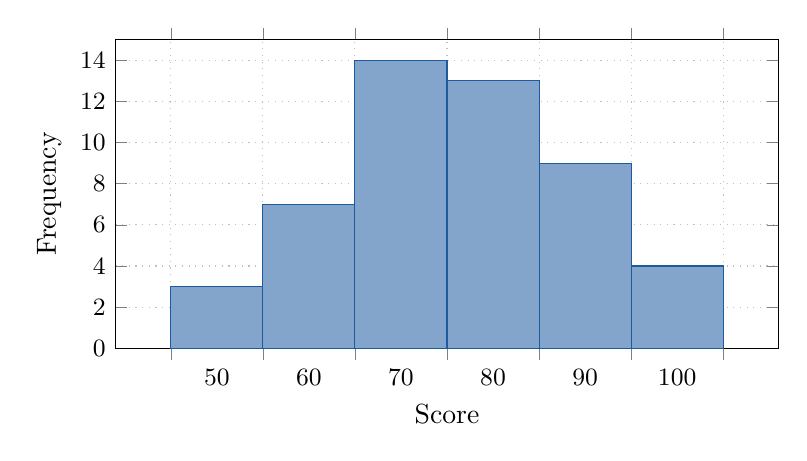
\begin{tikzpicture}
\begin{axis}[
  ybar interval,
  width=10cm, height=5.5cm,
  bar width=1.0,
  xtick={50,60,70,80,90,100,110},
  xticklabels={50,60,70,80,90,100,{}},
  x tick label style={font=\small},
  xlabel={Score},
  ylabel={Frequency},
  y tick label style={font=\small},
  ytick={0,2,4,6,8,10,12,14},
  ymin=0, ymax=15,
  ymajorgrids=true,
  grid style=dotted,
]
\addplot[fill=mathblue!55, draw=mathblue]
  coordinates {(50,3)(60,7)(70,14)(80,13)(90,9)(100,4)(110,0)};
\end{axis}
\end{tikzpicture}
\end{center}

The distribution is approximately symmetric and centered
near $75$--$80$.
Most scores fall between $60$ and $90$.
A small number of scores appear below $60$ or above $90$.
\end{example}

\begin{example}[Two distributions with the same mean]
The two distributions below both have mean $50$,
but different sample standard deviations.

\begin{center}
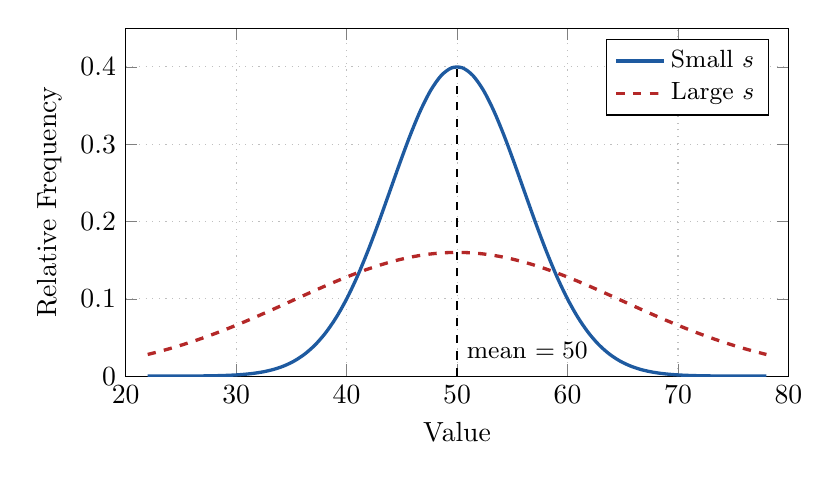
\begin{tikzpicture}
\begin{axis}[
  width=10cm, height=6cm,
  xlabel={Value},
  ylabel={Relative Frequency},
  ytick={0,0.1,0.2,0.3,0.4},
  ymin=0, ymax=0.45,
  xmin=20, xmax=80,
  grid=major,
  grid style=dotted,
  legend style={at={(0.97,0.97)}, anchor=north east, font=\small},
]
\addplot[mathblue, very thick, smooth, samples=60,
  domain=22:78]
  {0.40*exp(-0.5*((x-50)/6)^2)};
\addlegendentry{Small $s$}
\addplot[mathred, very thick, smooth, dashed, samples=60,
  domain=22:78]
  {0.16*exp(-0.5*((x-50)/15)^2)};
\addlegendentry{Large $s$}
\draw[black, thick, dashed]
  (axis cs:50,0) -- (axis cs:50,0.40);
\node[above right, font=\small] at (axis cs:50,0.01)
  {mean $= 50$};
\end{axis}
\end{tikzpicture}
\end{center}

The narrow distribution has a small sample standard deviation:
values cluster tightly around the mean.
The wide distribution has a large sample standard deviation:
values are spread broadly around the mean.
Both are centered at the same location.
\end{example}

\begin{exercises}
  \item The histogram below shows the distribution of
    heights (in inches) for a sample of 40 adults.

  \begin{center}
  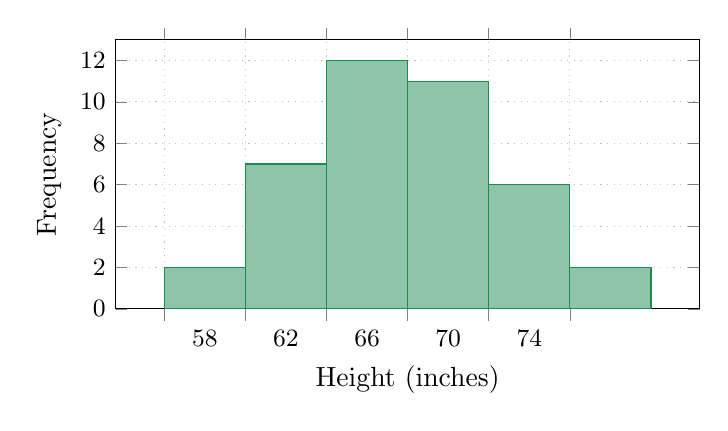
\begin{tikzpicture}
  \begin{axis}[
    ybar interval,
    width=9cm, height=5cm,
    bar width=1.0,
    xtick={58,62,66,70,74,78},
    xticklabels={58,62,66,70,74,{}},
    x tick label style={font=\small},
    xlabel={Height (inches)},
    ylabel={Frequency},
    y tick label style={font=\small},
    ytick={0,2,4,6,8,10,12},
    ymin=0, ymax=13,
    ymajorgrids=true,
    grid style=dotted,
  ]
  \addplot[fill=mathgreen!50, draw=mathgreen]
    coordinates {(58,2)(62,7)(66,12)(70,11)(74,6)(78,2)(82,0)};
  \end{axis}
  \end{tikzpicture}
  \end{center}

    \begin{enumerate}[label=(\alph*), itemsep=4pt]
      \item In which interval do most heights fall?
      \item Is the distribution symmetric or skewed?
      \item Would you expect the mean to be close to the
        median? Explain in one sentence.
    \end{enumerate}

  \item Sketch two histograms with the same center but
    different spreads. Label the center on both.
    Below each sketch, write one sentence describing
    what each distribution tells an observer about
    the data.

  \item A data set has mean $30$ and sample standard deviation $2$.
    A second data set has mean $30$ and sample standard deviation $8$.
    An observation of $36$ is taken.
    \begin{enumerate}[label=(\alph*), itemsep=4pt]
      \item How many sample standard deviations above the mean
        is $36$ in each data set?
      \item In which data set is the value $36$ more
        unusual? Explain in one sentence.
    \end{enumerate}
\end{exercises}

%--------------------------------------------------------------------
\section*{Chapter 3 Review}
%--------------------------------------------------------------------

\addcontentsline{toc}{section}{Chapter 3 Review}

\begin{enumerate}[label=\arabic*., leftmargin=2em, itemsep=8pt]

  \item The following data records the number of hours per
    week a sample of 10 students spend on homework:
    \[ 4,\; 7,\; 5,\; 8,\; 6,\; 5,\; 9,\; 4,\; 6,\; 6. \]
    \begin{enumerate}[label=(\alph*), itemsep=4pt]
      \item Find the mean, median, mode, and range.
      \item Construct the deviation table and compute
        the sample standard deviation.
      \item Describe the center and spread of this data
        set in two complete sentences.
    \end{enumerate}

  \item A company tracks the number of sick days taken
    by employees in one year.
    The data for eight employees is:
    \[ 0,\; 1,\; 2,\; 1,\; 0,\; 3,\; 1,\; 18. \]
    \begin{enumerate}[label=(\alph*), itemsep=4pt]
      \item Compute the mean and median.
      \item Which measure better represents a typical
        employee? Explain.
      \item If the value $18$ is removed, how do the mean
        and median each change? Compute both.
    \end{enumerate}

  \item Three students each score a mean of $80$ on five
    exams. Student A's scores are
    $78, 79, 80, 81, 82$.
    Student B's scores are
    $60, 70, 80, 90, 100$.
    Without computing, predict which student has the
    larger sample standard deviation.
    Then compute both sample standard deviations to verify.

  \item A data set has six values.
    Five of them are $12, 15, 14, 13, 16$.
    The mean of all six values is $14$.
    Find the sixth value.

  \item A histogram of test scores is skewed left.
    \begin{enumerate}[label=(\alph*), itemsep=4pt]
      \item What does it mean for a histogram to be
        skewed left?
      \item Would you expect the mean to be greater than,
        equal to, or less than the median?
        Explain in two sentences.
    \end{enumerate}

  \item The temperatures recorded over five days in two
    cities are:
    \begin{center}
    \renewcommand{\arraystretch}{1.4}
    \begin{tabular}{lrrrrr}
    \toprule
    & Day 1 & Day 2 & Day 3 & Day 4 & Day 5 \\
    \midrule
    City A & 68 & 70 & 69 & 71 & 67 \\
    City B & 55 & 62 & 74 & 79 & 85 \\
    \bottomrule
    \end{tabular}
    \end{center}
    \begin{enumerate}[label=(\alph*), itemsep=4pt]
      \item Compute the mean for each city.
      \item Compute the range and sample standard deviation
        for each city.
      \item Which city has more consistent temperatures?
        Justify using both spread measures.
    \end{enumerate}

  \item A quality control engineer samples 6 ball bearings
    and measures their diameters (in mm):
    \[ 9.98,\; 10.01,\; 10.00,\; 9.99,\; 10.02,\; 10.00. \]
    \begin{enumerate}[label=(\alph*), itemsep=4pt]
      \item Compute the mean and sample standard deviation.
      \item The specification requires that all bearings
        fall within $0.03$ mm of the target diameter of
        $10.00$ mm. Do all sampled bearings meet this
        requirement?
    \end{enumerate}

\end{enumerate}


\end{document}
